\subsection{制約付き最適化の条件を導く}

先に見た QP の KKT 条件は、二次関数とアフィン制約に限った特殊な公式ではない。滑らかな目的関数と滑らかな制約でも、最適点では目的関数の勾配が等式制約とアクティブな不等式制約の法線の組合せで打ち消される。

\begin{theorem}[KKT 条件]
制約付き最適化問題
\begin{align}
  \min_z\quad &J(z),\\
  \text{subject to}\quad &h(z)=0,\\
  &g(z)\le0
\end{align}
が適当な正則性条件を満たすとき、局所最適解 $z^*$ には乗数 $\lambda$、$\mu\ge0$ が存在して
\begin{align}
  \nabla J(z^*)+\nabla h(z^*)^\T\lambda+\nabla g(z^*)^\T\mu&=0,\\
  h(z^*)&=0,\\
  g(z^*)&\le0,\\
  \mu_i g_i(z^*)&=0
\end{align}
を満たす。これを Karush--Kuhn--Tucker 条件という。
\end{theorem}

\begin{derivation}
等式制約だけなら、制約面の上で $J$ が最小になる点では、許された微小変化方向に沿った $J$ の一次変化が 0 になる。これは $\nabla J$ が制約面の接空間に直交することを意味する。制約 $h(z)=0$ の法線方向は $\nabla h(z)$ で張られるので
\begin{equation}
  \nabla J(z)+\nabla h(z)^\T\lambda=0
\end{equation}
と書ける。不等式制約では、効いていない制約は局所的に無視できるので乗数が 0 になる。効いている制約では $g_i(z)=0$ で乗数が現れる。この二つを一つの式で表すのが
\begin{equation}
  \mu_i g_i(z)=0,
  \qquad
  \mu_i\ge0
\end{equation}
である。
\end{derivation}

\wfig{mpc-constraint-examples} の左図で、赤い二本の境界を $g_1(z)\le0$、$g_2(z)\le0$ とおくと、これらは制約付き最適点 $z^*$ が接している能動制約である。この点では
\begin{equation}
  \nabla J(z^*)+\mu_1\nabla g_1(z^*)+\mu_2\nabla g_2(z^*)=0
\end{equation}
となり、相補性 $\mu_i g_i(z^*)=0$ によって、赤い境界では $g_i(z^*)=0$ として正の乗数が目的関数の勾配を押し戻す。一方、赤くない境界は $g_j(z^*)<0$ の負のスラックを持つため、相補性を満たすには $\mu_j=0$ でなければならない。右図のように入力幅を狭くして入力制約が長く能動になり、その制約の乗数が大きな正の値を取る場合、局所応答を支配しているのは追従重みではなく制約余裕である。すなわち、MPC は目標へさらに近づく入力を選べても、許容入力幅を破らない方向へ解を押し戻している。

\subsection{線形 MPC の二次計画問題への定式化}

線形 MPC を数値ソルバへ渡すには、予測モデル、評価関数、制約を有限次元の行列問題としてそろえる。時刻 $k$ で利用できる状態推定値を $x_{k|k}$ と書き、予測中の状態と入力を
\begin{equation}
  x_{i|k}\simeq x_{k+i},
  \qquad
  u_{i|k}\simeq u_{k+i}
\end{equation}
と表す。線形時不変モデル
\begin{equation}
  x_{i+1|k}=Ax_{i|k}+Bu_{i|k},
  \qquad
  x_{0|k}=x_{k|k}
\end{equation}
を使うと、予測ホライズン $N_p$ に対する入力列と状態列は
\begin{equation}
  U=
  \begin{bmatrix}
    u_{0|k}\\u_{1|k}\\\vdots\\u_{N_p-1|k}
  \end{bmatrix},
  \qquad
  X=
  \begin{bmatrix}
    x_{1|k}\\x_{2|k}\\\vdots\\x_{N_p|k}
  \end{bmatrix}
\end{equation}
である。状態方程式を順に代入すると
\begin{equation}
  X=\mathcal{A}x_{k|k}+\mathcal{B}U
\end{equation}
を得る。ただし
\begin{equation}
  \mathcal{A}=
  \begin{bmatrix}
    A\\A^2\\\vdots\\A^{N_p}
  \end{bmatrix},
  \qquad
  \mathcal{B}=
  \begin{bmatrix}
    B&0&\cdots&0\\
    AB&B&\cdots&0\\
    \vdots&\vdots&\ddots&\vdots\\
    A^{N_p-1}B&A^{N_p-2}B&\cdots&B
  \end{bmatrix}
\end{equation}
である。このように状態列を現在状態と入力列のアフィン関数としてまとめる表現を、リフトアップした予測モデルという。

予測ホライズン $N_p$ は、何ステップ先まで状態と制約を評価するかを表す。一方、制御ホライズン $N_c$ は、何ステップ分の独立な入力移動を最適化するかを表し、ふつう $N_c\le N_p$ とする。$N_c=N_p$ なら上の $U$ の全成分を独立に選ぶ。$N_c<N_p$ では
\begin{equation}
  V=
  \begin{bmatrix}
    v_{0|k}\\v_{1|k}\\\vdots\\v_{N_c-1|k}
  \end{bmatrix}
\end{equation}
を真の決定変数とし、たとえば
\begin{equation}
  u_{i|k}=
  \begin{cases}
    v_{i|k}, & 0\le i<N_c,\\
    v_{N_c-1|k}, & N_c\le i<N_p
  \end{cases}
\end{equation}
のように最後の入力を保持する。この関係は $U=T_cV$ と書けるので、以下の QP は $U$ の代わりに $V$ を決定変数にしても同じ形を保つ。$N_p$ を長くすると遅い制約や終端集合を見やすくなるが、計算量が増える。$N_c$ を短くすると変数数は減るが、入力の自由度が減るため制約を避ける能力も下がる。

参照状態列と参照入力列を
\begin{equation}
  R_X=
  \begin{bmatrix}
    r_{1|k}\\r_{2|k}\\\vdots\\r_{N_p|k}
  \end{bmatrix},
  \qquad
  R_U=
  \begin{bmatrix}
    u^{\mathrm{ref}}_{0|k}\\u^{\mathrm{ref}}_{1|k}\\\vdots\\u^{\mathrm{ref}}_{N_p-1|k}
  \end{bmatrix}
\end{equation}
とする。終端コストを最後の状態へだけ置くなら、重み行列を
\begin{equation}
  \bar{Q}=\operatorname{blkdiag}(Q,\ldots,Q,P_f),
  \qquad
  \bar{R}=\operatorname{blkdiag}(R,\ldots,R)
\end{equation}
と定義できる。このとき評価関数
\begin{equation}
  J(U)=
  \frac{1}{2}(X-R_X)^\T \bar{Q}(X-R_X)
  +\frac{1}{2}(U-R_U)^\T \bar{R}(U-R_U)
\end{equation}
へリフトアップ表現を代入すると
\begin{equation}
  J(U)=\frac{1}{2}U^\T HU+g(x_{k|k})^\T U+\text{定数}
\end{equation}
となる。ただし
\begin{align}
  H&=\mathcal{B}^\T \bar{Q}\mathcal{B}+\bar{R},\\
  g(x_{k|k})&=\mathcal{B}^\T \bar{Q}(\mathcal{A}x_{k|k}-R_X)-\bar{R}R_U
\end{align}
である。$Q\ge0$、$P_f\ge0$、$R>0$ なら $\bar{R}>0$ なので $H>0$ であり、縮約した問題は狭義凸 QP として一意解を持つ。制御ホライズン $N_c<N_p$ の変数 $V$ を使う場合も、$U=T_cV$ の写像が列フルランクであれば $T_c^\T HT_c>0$ である。ただし、入力方向に正定な重みを置かない、または入力パラメータ化に冗長な自由度が残る場合には、ヘッセ行列が半正定値にとどまることもある。

状態制約、入力制約、終端制約も同じ手順で行列不等式になる。多面体制約を
\begin{align}
  G_xx_{i|k}&\le h_x,\\
  G_uu_{i|k}&\le h_u,\\
  G_fx_{N_p|k}&\le h_f
\end{align}
と書く。全時刻分を積み上げた行列を $\bar{G}_x$、$\bar{h}_x$、$\bar{G}_u$、$\bar{h}_u$ とし、最後の状態を選ぶ行列を
\begin{equation}
  E_f=
  \begin{bmatrix}
    0&0&\cdots&I
  \end{bmatrix}
\end{equation}
とおけば、縮約形式の制約は
\begin{equation}
  \begin{bmatrix}
    \bar{G}_u\\
    \bar{G}_x\mathcal{B}\\
    G_fE_f\mathcal{B}
  \end{bmatrix}U
  \le
  \begin{bmatrix}
    \bar{h}_u\\
    \bar{h}_x-\bar{G}_x\mathcal{A}x_{k|k}\\
    h_f-G_fE_f\mathcal{A}x_{k|k}
  \end{bmatrix}
\end{equation}
である。右辺だけが現在状態 $x_{k|k}$ に依存し、左辺の行列はモデルとホライズンが変わらなければ固定できる。状態列を消去しない疎形式では、決定変数を
\begin{equation}
  Z=
  \begin{bmatrix}
    x_{1|k}\\\vdots\\x_{N_p|k}\\u_{0|k}\\\vdots\\u_{N_p-1|k}
  \end{bmatrix}
\end{equation}
として、状態方程式を線形等式制約として残す。縮約形式は変数数が少ない一方で $H$ が密になりやすく、疎形式は変数数が多い一方で行列の帯構造を利用しやすい。

制約を常に守る必要がある場合、その制約はハード制約として残す。実行不可能性を避けたい性能制約では、スラック変数を導入してソフト制約にできる。たとえば状態制約を緩めるなら
\begin{align}
  \bar{G}_xX&\le\bar{h}_x+s,\\
  s&\ge0
\end{align}
を使い、決定変数を $\hat{U}=[U^\T\ s^\T]^\T$ に拡張する。評価関数へ
\begin{equation}
  \rho^\T s+\frac{1}{2}s^\T W_s s,
  \qquad
  \rho>0,
  \qquad
  W_s\ge0
\end{equation}
を加えると、制約違反は QP の中で数値的に最小化される。線形項 $\rho^\T s$ は小さな違反にも一定の罰を与え、二次項は大きな違反を強く抑える。入力の物理上限や安全上の不可侵集合は、ソフト制約にすると実機で守れない指令を最適解として許すため、通常はハード制約のまま扱う。

以上をまとめると、時刻 $k$ の線形 MPC はパラメータ $x_{k|k}$ を持つ QP
\begin{align}
  \min_{\hat{U}}\quad &
  \frac{1}{2}\hat{U}^\T \hat{H}\hat{U}
  +\hat{g}(x_{k|k})^\T \hat{U},\\
  \text{subject to}\quad &
  \hat{C}\hat{U}\le\hat{d}(x_{k|k}),\\
  &\hat{A}_{\mathrm{eq}}\hat{U}=\hat{b}_{\mathrm{eq}}(x_{k|k})
\end{align}
として書ける。縮約形式では等式制約が消えることもある。終端コスト $P_f$ はホライズンの先の価値を近似し、終端制約 $G_fx_{N_p|k}\le h_f$ は終端集合への到達を要求する。これらを置くと、前に述べた再帰的実行可能性と安定性の議論を QP の行列制約として実装できる。

後退ホライズン実装では、各サンプル時刻でこの QP を解き、最適列
\begin{equation}
  U^*_k=
  \begin{bmatrix}
    u^*_{0|k}\\u^*_{1|k}\\\vdots
  \end{bmatrix}
\end{equation}
の最初の入力 $u^*_{0|k}$ だけを対象へ加える。次の時刻では状態を測定または推定し直し、古い最適列を一つシフトした列を初期値として再び QP を解く。この繰返しにより、モデル誤差、外乱、推定誤差があっても、予測は毎回現在状態から作り直される。

一状態一入力の $N_p=2$ の形を明示する。$x_{i+1}=ax_i+bu_i$ とすると
\begin{equation}
  \begin{bmatrix}x_{1|k}\\x_{2|k}\end{bmatrix}
  =
  \begin{bmatrix}a\\a^2\end{bmatrix}x_{k|k}
  +
  \begin{bmatrix}
    b&0\\
    ab&b
  \end{bmatrix}
  \begin{bmatrix}u_{0|k}\\u_{1|k}\end{bmatrix}.
\end{equation}
$\bar{Q}=\operatorname{diag}(q,p_f)$、$\bar{R}=rI$、参照を 0 とすれば、$U=[u_{0|k}\ u_{1|k}]^\T$ に対する二次項と一次項は
\begin{align}
  H&=
  \begin{bmatrix}
    qb^2+p_fa^2b^2+r & p_fab^2\\
    p_fab^2 & p_fb^2+r
  \end{bmatrix},\\
  g(x_{k|k})&=
  \begin{bmatrix}
    qab+p_fa^3b\\
    p_fa^2b
  \end{bmatrix}x_{k|k}
\end{align}
である。さらに $\abs{x_{i|k}}\le x_{\max}$、$\abs{u_{i|k}}\le u_{\max}$ を課すと、入力制約は $U$ の上下限になり、状態制約は
\begin{equation}
  -x_{\max}\mathbf{1}
  \le
  \begin{bmatrix}a\\a^2\end{bmatrix}x_{k|k}
  +
  \begin{bmatrix}
    b&0\\
    ab&b
  \end{bmatrix}U
  \le
  x_{\max}\mathbf{1}
\end{equation}
となる。これは現在状態で右辺が変わる線形不等式であり、線形 MPC が各サンプルで解く QP の最小構成を表している。

この縮約形式は、\wfig{mpc-architecture} の最適化器が各サンプルで作る数値問題そのものである。予測モデルと制約集合は固定行列を与え、推定状態 $\hat{x}_k$ と参照値は一次項と右辺を更新し、\wfig{mpc-constraint-examples} の可行集合と能動制約を決める。したがって、線形 MPC の実装確認では、制御則の式だけでなく、行列の寸法、現在状態に依存する右辺、ソルバが返す制約違反を同時に見る。

この例では、QP データのうち現在状態に依存する部分を直接切り分けられる。$\Phi=\begin{bmatrix}a&a^2\end{bmatrix}^\T$、$\Gamma=\begin{bmatrix}b&0\\ab&b\end{bmatrix}$ とおくと、状態制約は
\begin{equation}
  \begin{bmatrix}
    \Gamma\\-\Gamma
  \end{bmatrix}U
  \le
  \begin{bmatrix}
    x_{\max}\mathbf{1}-\Phi x_{k|k}\\
    x_{\max}\mathbf{1}+\Phi x_{k|k}
  \end{bmatrix}
\end{equation}
である。モデル、重み、ホライズン、制約形を固定したまま $x_{k|k}$ を大きくしても、$H$ は固定された予測行列と重みから決まるため変わらない。一方、自由応答 $\Phi x_{k|k}$ が変わるので、$g(x_{k|k})$ と状態制約の右辺は変わる。左辺の制約行列 $\Gamma$、$-\Gamma$、および入力制約の $\pm I$ は、固定したモデルとホライズンでは変わらない。この分離をログで追うと、毎サンプルで更新すべきデータだけが更新され、固定してよい行列を誤って作り替えていないことを確認できる。

\wfig{mpc-constraint-examples} の右図のように入力幅 $u_{\max}$ を狭くすると、入力制約の右辺も小さくなり、可行集合は入力上下限から先に削られる。このとき QP ログに最大制約違反を残すと、予測状態または入力が許容範囲を超えた実行不能化や制約実装の符号誤りを検出できる。能動制約の一覧は、閉ループが状態上限で止められているのか、入力飽和で追従を諦めているのかを示す。KKT 残差は、可行に見える解でも数値収束が不十分で最適性条件を満たしていない失敗を露出させる。最後に適用入力 $u^*_{0|k}$ を時系列で記録すると、ホライズン内の先頭要素を取り違える実装ミス、飽和付近のチャタリング、想定した能動制約と実際の入力符号が合わない異常を閉ループ応答として追跡できる。

\subsection{非線形 MPC の直接法と実時間反復法}

線形 MPC では、予測モデルがアフィンで、評価関数が二次形式であり、制約が線形不等式として積み上がるため、各サンプルの問題は QP になる。これに対して、対象の運動方程式、アクチュエータ特性、座標変換、抵抗、摩擦、幾何制約をそのまま使うと、予測モデルは非線形になる。サンプル時刻 $t_k$ での状態推定値を $\hat{x}_k$ とし、連続時間の非線形モデルを
\begin{equation}
  \dot{x}(t)=f(x(t),u(t),p),
  \qquad
  y(t)=h(x(t),u(t),p)
\end{equation}
と書く。$p$ は質量、時定数、抵抗係数などのパラメータである。非線形 MPC は、有限時間区間 $[t_k,t_k+T]$ 上で
\begin{align}
  \min_{x(\cdot),u(\cdot),s(\cdot)}\quad &
  \int_{t_k}^{t_k+T}
  \ell(x(t),u(t),r(t),s(t))\,\dd t
  +V_f(x(t_k+T),r_f),\\
  \text{subject to}\quad &
  \dot{x}(t)=f(x(t),u(t),p),\\
  &x(t_k)=\hat{x}_k,\\
  &c(x(t),u(t),s(t))\le0,\\
  &s(t)\ge0,\qquad
  c_f(x(t_k+T))\le0
\end{align}
を解く。$r(t)$ は参照軌道、$s(t)$ は緩和可能な制約にだけ入れるスラック変数である。典型的な一段コストは
\begin{equation}
  \ell(x,u,r,s)
  =\frac{1}{2}\norm{x-r_x}_{Q}^{2}
  +\frac{1}{2}\norm{u-r_u}_{R}^{2}
  +\rho^\T s+\frac{1}{2}s^\T W_s s
\end{equation}
である。ただし $\norm{v}_{Q}^{2}=v^\T Qv$ とする。安全上越えてはならない状態制約や物理的な入力上下限は、線形 MPC と同様にハード制約として残す。ソフト制約は、追従誤差や快適性のように、違反量を明示的に罰すれば閉ループを止めずに扱える制約へ限って使う。

連続時間の最適制御問題をそのまま計算機で解くことはできないので、時間区間を
\begin{equation}
  t_k=\tau_0<\tau_1<\cdots<\tau_N=t_k+T
\end{equation}
に分け、関数 $x(t)$ と $u(t)$ を有限個の変数へ置き換える。このように、状態と入力の関数空間を有限次元の非線形計画問題へ直接変換する方法を直接法という。ポントリャーギンの最小原理から境界値問題を作る間接法と違い、直接法では状態制約、入力制約、スラック、終端制約を最適化問題の制約としてそのまま持ち込めるため、MPC 実装で広く使われる。

直接単一射撃法では、決定変数を入力パラメータだけにする。各区間で入力を一定、または低次多項式で表し、
\begin{equation}
  U=
  \begin{bmatrix}
    u_0\\u_1\\\vdots\\u_{N-1}
  \end{bmatrix}
\end{equation}
を選ぶと、状態列は初期値 $\hat{x}_k$ から数値積分によって一意に決まる。
\begin{equation}
  x_{i+1}=\Phi_i(x_i,u_i),
  \qquad
  x_0=\hat{x}_k
\end{equation}
ここで $\Phi_i$ は区間 $[\tau_i,\tau_{i+1}]$ の数値積分写像である。単一射撃法の利点は変数数が少ないことである。しかし、初期の入力が全ホライズンの状態に強く影響するため、長いホライズンや不安定なモデルでは感度が大きくなり、制約違反の情報が入力列へ戻りにくい。途中状態を明示変数として持たないので、遠い時刻の状態制約を満たす方向を見つけるまでに反復が不安定になることがある。

直接多重射撃法では、各節点の状態も決定変数に含める。
\begin{equation}
  Z=
  \begin{bmatrix}
    x_0\\x_1\\\vdots\\x_N\\u_0\\u_1\\\vdots\\u_{N-1}
  \end{bmatrix}
\end{equation}
初期条件と各区間の連続性は
\begin{align}
  x_0-\hat{x}_k&=0,\\
  x_{i+1}-\Phi_i(x_i,u_i)&=0
  \qquad (i=0,\ldots,N-1)
\end{align}
として課す。二つ目の等式は、節点変数 $x_{i+1}$ と、前の節点から数値積分して得た状態が一致することを要求する欠陥制約である。欠陥が 0 でない間は、節点をつないだ軌道は物理モデルを満たしていない。最適化は、評価関数を下げるだけでなく、すべての欠陥を 0 へ戻す方向も同時に探す。多重射撃法は変数数と等式制約数が増えるが、状態制約を節点で直接扱え、長いホライズンでも感度が局所化される。

直接コロケーション法では、各区間内の状態軌道を多項式で近似し、微分方程式を選ばれた内部点で満たすようにする。区間 $[\tau_i,\tau_{i+1}]$ の幅を $h_i=\tau_{i+1}-\tau_i$ とし、正規化時間 $\theta\in[0,1]$ 上で
\begin{equation}
  x(t)\simeq X_i(\theta)
  =\sum_{j=0}^{d}L_j(\theta)x_{i,j},
  \qquad
  u(t)\simeq U_i(\theta)
\end{equation}
とおく。$L_j$ は補間多項式であり、$x_{i,j}$ は区間内の節点または内部点の状態変数である。コロケーション点 $\theta_m$ で微分方程式を満たす条件は
\begin{equation}
  \frac{1}{h_i}\frac{\dd X_i}{\dd\theta}(\theta_m)
  -f(X_i(\theta_m),U_i(\theta_m),p)=0
  \qquad (m=1,\ldots,d)
\end{equation}
である。区間の終端では、補間多項式の終端値と次の節点状態を一致させる欠陥制約
\begin{equation}
  x_{i+1}-X_i(1)=0
\end{equation}
も置く。コロケーション法は数値積分を最適化問題の内部へ展開するため、微分方程式、経路制約、終端制約が大きな疎な NLP として現れる。滑らかな軌道制約や硬い微分方程式を扱いやすい一方、変数数は多く、離散化点、コロケーション次数、スケーリングの選び方が数値性を大きく左右する。

直接法で得られる非線形計画問題を
\begin{align}
  \min_z\quad &J(z),\\
  \text{subject to}\quad &F(z)=0,\\
  &G(z)\le0
\end{align}
と書く。ここで $z$ は入力列、節点状態、コロケーション点、スラックをまとめた変数である。逐次二次計画法、すなわち SQP は、現在の反復点 $z^j$ のまわりで制約を一次近似し、ラグランジアン
\begin{equation}
  \mathcal{L}(z,\lambda,\mu)
  =J(z)+\lambda^\T F(z)+\mu^\T G(z)
\end{equation}
の曲率を二次近似して、ステップ $\Delta z$ に関する QP を作る。等式制約は
\begin{equation}
  F(z^j)+F_z(z^j)\Delta z=0
\end{equation}
へ、不等式制約は
\begin{equation}
  G(z^j)+G_z(z^j)\Delta z\le0
\end{equation}
へ線形化される。目的関数は
\begin{equation}
  J(z^j+\Delta z)
  \simeq
  J(z^j)+\nabla J(z^j)^\T\Delta z
  +\frac{1}{2}\Delta z^\T B^j\Delta z
\end{equation}
と二次化する。$B^j$ はラグランジアンヘッセ行列 $\nabla_{zz}^{2}\mathcal{L}(z^j,\lambda^j,\mu^j)$ の近似である。最小二乗型の NMPC では、残差 $r(z)$ に対して
\begin{equation}
  J(z)=\frac{1}{2}\norm{r(z)}^2
\end{equation}
と書ける部分が多い。このとき
\begin{equation}
  \nabla^2 J(z)
  =J_r(z)^\T J_r(z)
  +\sum_\alpha r_\alpha(z)\nabla^2 r_\alpha(z)
\end{equation}
であり、残差が小さい運転点では第二項を無視して
\begin{equation}
  B^j\simeq J_r(z^j)^\T J_r(z^j)
\end{equation}
とする Gauss--Newton 近似がよく使われる。これは正半定値の曲率を作りやすく、QP の数値解法と相性がよい。ただし、残差が大きい、強い非線形制約が効く、または不安定な初期値から始める場合には、厳密ヘッセ行列、準 Newton 更新、正則化、信頼領域が必要になる。

\subsubsection{非線形最小二乗構造と Gauss--Newton 近似}

NMPC の追従コストは、多くの場合、状態偏差、入力偏差、入力変化、スラック変数を残差として積み上げた非線形最小二乗問題で表せる。たとえば直接多重射撃法の決定変数を
\begin{equation}
  z=
  (x_0,\ldots,x_N,u_0,\ldots,u_{N-1},s_0,\ldots,s_N)
\end{equation}
とし、重みの平方根を $Q_i^{1/2}$、$R_i^{1/2}$、$W_{s,i}^{1/2}$ と書くと、残差ベクトルを
\begin{equation}
  r(z)=
  \begin{bmatrix}
    Q_0^{1/2}(x_0-r_{x,0})\\
    R_0^{1/2}(u_0-r_{u,0})\\
    W_{s,0}^{1/2}s_0\\
    \vdots\\
    P_f^{1/2}(x_N-r_{x,N})
  \end{bmatrix}
\end{equation}
のように定義できる。このとき評価関数は
\begin{equation}
  J(z)=\frac{1}{2}r(z)^\T r(z)
\end{equation}
である。現在の反復点 $z^j$ からの変化を $\Delta z$ とし、残差のヤコビアンを
\begin{equation}
  R_z^j=\frac{\pp r}{\pp z}(z^j)
\end{equation}
とおけば、一次近似
\begin{equation}
  r(z^j+\Delta z)\simeq r^j+R_z^j\Delta z
\end{equation}
から、ステップに関する二次近似
\begin{align}
  \frac{1}{2}\norm{r^j+R_z^j\Delta z}^{2}
  &=
  \frac{1}{2}\Delta z^\T (R_z^j)^\T R_z^j\Delta z
  +\{(R_z^j)^\T r^j\}^\T\Delta z
  +\frac{1}{2}(r^j)^\T r^j
\end{align}
を得る。したがって QP へ入る勾配とヘッセ行列近似は
\begin{equation}
  g_{\mathrm{GN}}^j=(R_z^j)^\T r^j,
  \qquad
  B_{\mathrm{GN}}^j=(R_z^j)^\T R_z^j
\end{equation}
である。$B_{\mathrm{GN}}^j$ は常に半正定値なので、厳密な二階微分に由来する負の曲率を QP へ直接入れずにすむ。

Gauss--Newton 近似が捨てている項は、残差そのものに比例する。成分表示で書けば
\begin{equation}
  \nabla^2J(z)
  =
  R_z(z)^\T R_z(z)
  +\sum_{\alpha=1}^{n_r}r_\alpha(z)\nabla^2r_\alpha(z)
\end{equation}
である。第二項は、参照追従がよく達成され、モデル誤差や制約違反が小さい近傍では小さい。一方、大きなステップ状参照、強い非線形出力、摩擦や飽和を含むモデル、悪いウォームスタート、または経済 MPC のように最小二乗でない目的を含む場合には、この項が探索方向を大きく変える。非線形等式制約や不等式制約の曲率も、本来はラグランジアンヘッセ行列
\begin{equation}
  \nabla_{zz}^{2}\mathcal{L}
  =
  \nabla^2J
  +\sum_i\lambda_i\nabla^2F_i
  +\sum_j\mu_j\nabla^2G_j
\end{equation}
へ入る。制約乗数が大きいアクティブ制約では、目的関数の残差が小さくても制約曲率を無視できないことがある。その場合は厳密ヘッセ行列、BFGS 型の準 Newton 更新、または
\begin{equation}
  B^j=(R_z^j)^\T R_z^j+\rho I,
  \qquad
  \rho>0
\end{equation}
のような Levenberg--Marquardt 型正則化を使い、直線探索や信頼領域で全ステップを抑える。

一変数の小例で第二項の意味を確認する。状態 $x$ はここでは定数として扱い、非線形出力残差を
\begin{equation}
  r_1(u)=x-\sin u,
  \qquad
  r_2(u)=\sqrt{\rho}\,u
\end{equation}
とする。評価関数は
\begin{equation}
  J(u)=\frac{1}{2}(x-\sin u)^2+\frac{\rho}{2}u^2
\end{equation}
であり、厳密な二階微分は
\begin{equation}
  \frac{\dd^2J}{\dd u^2}
  =
  \cos^2u+(x-\sin u)\sin u+\rho
\end{equation}
である。Gauss--Newton 近似は
\begin{equation}
  B_{\mathrm{GN}}=\cos^2u+\rho
\end{equation}
だけを使う。$x-\sin u$ が小さければ両者は近いが、追従残差が大きい初期反復では $(x-\sin u)\sin u$ が曲率の符号や大きさに効く。したがって、Gauss--Newton 近似は「常に厳密な Newton 法の代替」ではなく、残差が十分小さい最小二乗構造を利用した実時間向きの近似である。

\subsubsection{微分計算、疎構造、終了判定の実装}

SQP や RTI の計算量は、関数値そのものよりも、ヤコビアンとヘッセ行列近似をどのように作るかで決まる。有限差分は、関数評価を繰り返して
\begin{equation}
  \frac{\pp \phi}{\pp z_i}(z)
  \simeq
  \frac{\phi(z+\epsilon e_i)-\phi(z)}{\epsilon}
\end{equation}
と近似する方法である。実装は簡単だが、前進差分でも変数数 $n_z$ に比例した追加評価が必要であり、$\epsilon$ が大きいと打切り誤差、小さいと丸め誤差が支配的になる。中心差分は精度を上げるが、おおよそ $2n_z$ 回の追加評価を要する。記号微分、すなわちシンボリック微分は式として正確な微分を与えるが、長いホライズン、条件分岐、外部関数、表引き、飽和を含む実装では式が肥大化し、コードの保守が難しくなる。

自動微分は、実装された計算手順を基本演算の合成として扱い、連鎖律を機械的に適用して微分を得る。方向 $v$ に沿う順方向微分は
\begin{equation}
  J_\phi(z)v
  =
  \left.\frac{\dd}{\dd\epsilon}\phi(z+\epsilon v)\right|_{\epsilon=0}
\end{equation}
を一回の計算伝播で求める。逆方向微分は、重み $w$ に対する
\begin{equation}
  J_\phi(z)^\T w
\end{equation}
を効率よく求める。状態次元、入力次元、制約本数、残差本数のどれが大きいかに応じて順方向と逆方向を選ぶ。自動微分は有限差分の刻み幅調整を不要にし、実装コードと微分コードの不一致を減らせる。一方、条件分岐、不連続な飽和、表の補間、数値積分器の内部反復を含む場合には、どの分岐の微分を取っているか、滑らかでない点をどのように扱うかを明示しなければならない。

直接多重射撃法の線形化は、疎構造を持つ。各区間の欠陥制約
\begin{equation}
  F_i(z)=x_{i+1}-\Phi_i(x_i,u_i)=0
\end{equation}
の微分は
\begin{equation}
  \Delta x_{i+1}
  -A_i\Delta x_i
  -B_i\Delta u_i
  =-F_i(z^j),
  \qquad
  A_i=\frac{\pp\Phi_i}{\pp x_i},
  \quad
  B_i=\frac{\pp\Phi_i}{\pp u_i}
\end{equation}
であり、隣り合う節点と入力にしか結合しない。この帯構造を残す疎形式では、変数数は多いが KKT 行列の非ゼロ要素が局所的に並ぶ。状態増分を再帰的に消去する縮約、すなわち condensing では
\begin{equation}
  \Delta x_i
  =
  \Phi_{i,0}\Delta x_0
  +\sum_{j=0}^{i-1}\Phi_{i,j+1}B_j\Delta u_j
  +d_i
\end{equation}
のように $\Delta x_i$ を入力増分で表し、QP の変数を $\Delta U$ へ減らす。全縮約は短いホライズンで有効だが、ヘッセ行列と制約行列が密になりやすい。長いホライズンや高次元状態では、疎形式または一部だけをまとめる部分縮約により、線形代数の時間とメモリを抑える。どの形式が速いかは、変数数だけでなく、帯幅、制約数、キャッシュ、分解の再利用、ウォームスタートされたアクティブ集合に依存する。

ウォームスタートでは、前回の入力列を一つシフトするだけでなく、状態列、スラック、等式乗数、不等式乗数、内点法のスラックとバリア変数も同じ時刻対応へ移す。多重射撃法では、シフトした状態列をそのまま使うと欠陥が残るので、必要に応じて新しい初期状態から短い再積分を行い、欠陥制約の残差を小さくしてから線形化する。乗数の符号やアクティブ集合を持ち越すと QP の反復数は減りやすいが、参照や制約が急に変わったときには古い乗数が誤った面へ反復を引き寄せるため、最大値で切る、古いアクティブ集合を一度緩める、といった初期化を入れる。

終了判定は、ソルバ内部の無次元な数値だけで決めず、スケーリング後の残差と物理単位での違反量を併記する。代表的には、停留残差、等式制約残差、不等式制約違反、相補性を
\begin{align}
  r_{\mathrm{stat}}
  &=\nabla J(z)+F_z(z)^\T\lambda+G_z(z)^\T\mu,\\
  r_{\mathrm{eq}}&=F(z),\\
  r_{\mathrm{ineq}}&=\max\{0,G(z)\},\\
  r_{\mathrm{comp}}&=\mu\circ G(z)
\end{align}
として監視する。許容値は絶対許容値だけでなく、問題のスケールに対する相対許容値も持たせる。
\begin{equation}
  \norm{r_{\mathrm{eq}}}_\infty
  \le
  \epsilon_{\mathrm{abs}}
  +\epsilon_{\mathrm{rel}}\max\{1,\norm{z}_\infty\}
\end{equation}
のような判定は、単位や変数スケールが変わったときに同じ意味を保ちやすい。ただし、最終的には温度なら [$^\circ$C]、位置なら [m]、入力なら [N] や [V] の違反量として、ハード制約の余裕より小さいかを確認する必要がある。

実時間実装では、最適性の許容値より先に締切が存在する。制御周期 $T_s$ に対して、測定、推定、問題生成、QP 解法、通信、監視にかかる時間を
\begin{equation}
  T_{\mathrm{meas}}+T_{\mathrm{est}}+T_{\mathrm{form}}
  +T_{\mathrm{solve}}+T_{\mathrm{comm}}+T_{\mathrm{mon}}
  \le T_s-T_{\mathrm{margin}}
\end{equation}
へ収める。締切を過ぎてから返った最適入力は、古い状態に対する入力であり、採用条件を満たさない。したがって実装では、反復回数上限、時間上限、途中で得られた可行点、前回有効解、安全側入力を明確に区別する。制限時間で打ち切った場合、ハード制約を満たす可行点が得られているなら劣化運転として採用できる可能性があるが、可行性が確認できない点を「ほぼ最適」として対象へ入れてはならない。

ソルバ実装の確認は、閉ループ実験の前に単体で行う。第一に、自動微分で得た方向微分を有限差分で検査し、
\begin{equation}
  \frac{\norm{\phi(z+\epsilon v)-\phi(z)-\epsilon J_\phi(z)v}}
       {\epsilon\max\{1,\norm{\phi(z)}\}}
\end{equation}
が $\epsilon$ を変えたときに期待した次数で小さくなるかを見る。第二に、線形化 QP の解 $\Delta z$ を元の非線形制約へ戻し、実際の $F(z+\Delta z)$、$G(z+\Delta z)$ が許容範囲に入るかを確認する。第三に、冷スタート、通常のウォームスタート、参照急変、センサ外れ値、制約境界、最大ホライズン、最悪ジッタで、計算時間、終了状態、最大制約違反、KKT 残差、採用された入力をログに残す。これらの検査により、微分、疎構造、縮約、終了判定、締切処理が同じ最適化問題を指していることを確認できる。

SQP の一反復で解く QP は
\begin{align}
  \min_{\Delta z}\quad &
  \frac{1}{2}\Delta z^\T B^j\Delta z+\nabla J(z^j)^\T\Delta z,\\
  \text{subject to}\quad &
  F(z^j)+F_z(z^j)\Delta z=0,\\
  &G(z^j)+G_z(z^j)\Delta z\le0
\end{align}
である。QP の解をそのまま $z^{j+1}=z^j+\Delta z$ とするとは限らない。非線形制約の近似が粗いと、全ステップは実際の NLP の制約違反や評価関数を悪化させる。そこで直線探索では
\begin{equation}
  z^{j+1}=z^j+\alpha\Delta z,
  \qquad
  0<\alpha\le1
\end{equation}
とし、メリット関数が下がる $\alpha$ を選ぶ。信頼領域法では $\norm{\Delta z}\le\Delta_{\max}$ のような半径を置き、線形化と二次化が信用できる範囲に QP を制限する。MPC ではサンプル時刻が進むため、完全収束だけを目標にすると計算時間を超えることがある。この点が、オフラインの非線形最適化と実時間 NMPC の違いである。

実時間反復法、すなわち RTI は、各サンプル時刻で SQP を完全収束させず、一回の線形化、一回の QP 解法、一回の更新だけを行う考え方である。時刻 $k-1$ で得た軌道
\begin{equation}
  z^*_{k-1}
  =
  (x^*_{0|k-1},\ldots,x^*_{N|k-1},
   u^*_{0|k-1},\ldots,u^*_{N-1|k-1})
\end{equation}
を一つ前へシフトし、最後に終端制御則、定常入力、または最後の入力保持を付けて、時刻 $k$ の初期軌道 $\bar{z}_k$ を作る。これをウォームスタートという。測定または推定された新しい初期状態 $\hat{x}_k$ を反映し、必要なら多重射撃区間の欠陥を小さくしてから、$\bar{z}_k$ のまわりでモデルと制約を線形化して QP を解く。得られたステップ $\Delta z_k$ で
\begin{equation}
  z_k^+=\bar{z}_k+\Delta z_k
\end{equation}
を作り、その最初の入力 $u_{0|k}^+$ だけを対象へ加える。次のサンプルでは、$z_k^+$ を再びシフトして使う。RTI の要点は、閉ループが短い周期で同じ最適化問題の近傍を追い続けるなら、毎回 NLP を厳密に解き切らなくても、前回解からの一 QP ステップで十分な改善が得られるという点にある。

ウォームスタートには、入力列だけでなく、状態列、等式制約の乗数、不等式制約の乗数、アクティブ集合、内点法のバリア変数も含められる。線形 MPC の QP でもシフト初期値は有効であるが、NMPC では初期値の質がさらに重要である。非線形モデルでは、初期軌道が力学から大きく外れていると、欠陥制約の線形化が現実的な修正方向を与えない。多重射撃法では、シフト後に各区間を再積分して欠陥を小さくする準備段階を置くことがある。コロケーション法では、補間多項式を時間方向へ移し、終端側を定常値または局所フィードバックで延長する。

NMPC では実行可能性の扱いが線形 MPC より繊細である。非線形制約を一次近似した QP が実行不可能になることは、元の NLP が実行不可能であることを必ずしも意味しない。線形化点が悪い、スケーリングが悪い、あるいはハード制約の余裕が極端に小さいだけでも QP は破綻する。実装では、まず物理入力上限や安全制約を破らない範囲で、状態経路制約にスラックを入れる。次に、評価関数よりも制約違反の減少を優先する復旧問題を解く。例えば
\begin{align}
  \min_{z,s}\quad &
  \frac{1}{2}\norm{s}^{2}
  +\frac{\eta}{2}\norm{z-\bar{z}}^{2},\\
  \text{subject to}\quad &
  F(z)=0,\\
  &G_{\mathrm{hard}}(z)\le0,\\
  &G_{\mathrm{soft}}(z)\le s,\qquad s\ge0
\end{align}
のような問題は、元の追従性能よりも可行性の回復を優先する。これを restoration、または実行可能性回復の段階という。回復してもハード制約を満たす入力が見つからない場合には、NMPC の外側に、入力遮断、制限付き保持、低ゲイン制御、非常停止などの安全側制御を置く必要がある。最適化ソルバの成功判定だけに安全を委ねるべきではない。

線形 MPC と NMPC の実務上の差は、表現力、保証、計算量の交換である。線形 MPC は、モデルと制約を一度行列問題へ変換すれば、各サンプルで凸 QP を解くため、大域最適性、実行可能性、終端条件に基づく安定性を解析しやすい。モデル誤差が小さい運転範囲、制約が主に入力上下限と線形状態制約で表せる場合、線形 MPC は実装と検証が容易である。一方、NMPC は、広い運転範囲、強い非線形性、状態依存の制約、座標や姿勢を含むモデル、入力と状態が非線形に結合する対象を直接扱える。しかし、得られる問題は一般に非凸であり、解は局所最適にとどまり、初期値、スケーリング、離散化、ソルバの終了条件に閉ループ性能が依存する。

したがって、NMPC を選択する根拠は手法の高度さではなく、線形近似では制約や予測誤差が支配的になるほど非線形性が重要であることに置く。線形 MPC で十分な余裕があるなら、計算時間、検証、保守性の点で線形 MPC が有利である。NMPC を用いる場合には、モデル評価時間、ヤコビアン計算、自動微分、スケーリング、ウォームスタート、失敗時の入力、制約回復、ログによる残差監視までを制御器の一部として設計する。理論上の最適性よりも、各サンプルで制約を破らず、制限時間内に有効な入力を返すことが、実時間 NMPC の中心条件である。

したがって、NMPC の確認は新しい数値解法だけを評価する作業ではない。\wfig{mpc-architecture} の最適化器が、非線形モデル、制約、推定状態を受け取り、制限時間内に採用可能な先頭入力を返したかを確認する作業である。採用条件は、\wfig{implementation-effects-examples} で見た実入力と制約余裕の検査へ直接接続する。

直接多重射撃法で一つの RTI サンプルを検証すると、処理順は次の連鎖になる。まず、前回の $z^*_{k-1}$ を一つ前へシフトし、終端側を終端制御則、定常入力、または最後の入力保持で延長して $\bar{z}_k$ を作る。次に、先頭状態を測定または推定値で置き換えて $x_{0|k}=\hat{x}_k$ を課す。この置換で多重射撃の欠陥
\begin{equation}
  d_i(\bar{z}_k)
  =
  x_{i+1|k}-\Phi_i(x_{i|k},u_{i|k})
\end{equation}
が大きくなった場合には、区間の再積分や局所補正で $\max_i\norm{d_i(\bar{z}_k)}$ を前処理許容値まで下げる。その準備済み軌道のまわりで力学と経路制約を線形化し、線形化 QP を一回解き、得られた $\Delta z_k$ から $z_k^+=\bar{z}_k+\Delta z_k$ を作る。ここで適用候補になるのは軌道全体ではなく、先頭入力 $u^+_{0|k}$ だけである。

一回の SQP ステップで得た $u^+_{0|k}$ は、滑らかな入力列に見えても、そのまま採用可能とは限らない。採用可能な入力は、元の非線形制約へ戻して評価したハード制約違反
\begin{equation}
  v_{\mathrm{hard}}
  =
  \max_\ell \max\{0,G_{\mathrm{hard},\ell}(z_k^+)\}
\end{equation}
が許容値以下であり、最大欠陥残差
\begin{equation}
  r_{\mathrm{def}}
  =
  \max_i\norm{x^+_{i+1|k}-\Phi_i(x^+_{i|k},u^+_{i|k})}
\end{equation}
も許容値以下であり、QP と後処理が計算締切 $T_{\mathrm{dead}}$ 内に終わり、監視フラグが正常である場合に限られる。逆に、ハード制約違反が残る入力、欠陥残差が大きく予測軌道として信用できない入力、締切後に返ってきた入力、数値発散、スケーリング異常、センサ外れ値、復旧段階への遷移などを示す監視フラグ付きの入力は、SQP が一回進んでいても非採用である。この場合は、前回の実行可能入力の制限付き保持、低ゲイン制御、入力遮断など、外側の安全側制御へ切り替える。

\begin{figure}[tbp]
  \centering
  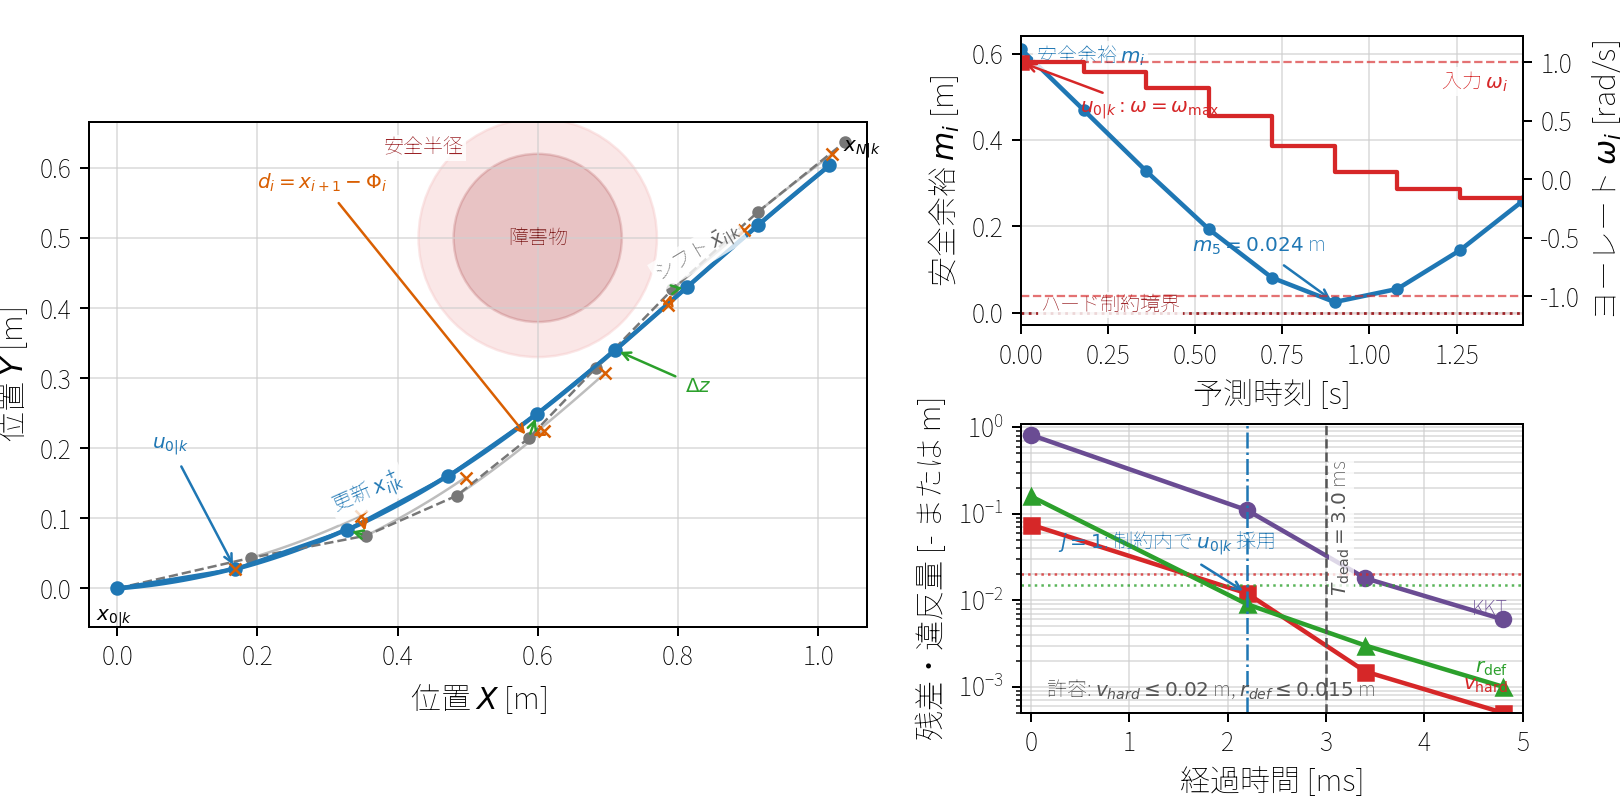
\includegraphics[width=0.96\linewidth,bb=0 0 648 324]{figures/w07_nmpc_mesh_solver_horizon.png}
  \caption{直接多重射撃法で見た NMPC のメッシュ、後退ホライズン、ソルバ監視量。左はシフト後の節点 $\bar{x}_{i|k}$、区間積分 $\Phi_i(\bar{x}_{i|k},\bar{u}_{i|k})$、欠陥 $d_i$、RTI ステップ $\Delta z$、更新後の予測節点 $x^+_{i|k}$ を同じ平面上に重ねる。右上は障害物安全半径に対する状態余裕 $m_i$ とヨーレート入力 $\omega_i$ を示し、先頭入力 $u_{0|k}$ が入力上限で能動になっていることを示す。右下は KKT 停留残差、ハード制約違反 $v_{\mathrm{hard}}$、欠陥残差 $r_{\mathrm{def}}$、締切 $T_{\mathrm{dead}}$ を同じサンプルの採用判定として並べる。}
  \label{fig:w07-nmpc-mesh-solver-horizon}
\end{figure}

\wfig{w07-nmpc-mesh-solver-horizon} の左図では、節点を単に滑らかな線で結ぶだけでは直接法の検証にならないことが分かる。灰色のシフト軌道 $\bar{x}_{i|k}$ は前回解から作った初期値であり、各区間を非線形モデルで積分した点 $\Phi_i(\bar{x}_{i|k},\bar{u}_{i|k})$ と次節点のずれが欠陥 $d_i$ である。RTI の $\Delta z$ は追従誤差を小さくするだけでなく、この欠陥を物理モデルに沿う連続軌道へ戻す修正として解釈する。したがって、予測経路の形、節点、区間、欠陥矢印を同時に残すと、ソルバがきれいな入力列を返しただけなのか、力学制約を満たす予測を返したのかを分離できる。

右上のホライズン表示では、障害物中心からの距離に安全半径を引いた余裕 $m_i$ を [m] で読み、入力列の先頭 $u_{0|k}$ を同じ時刻のヨーレート上限と照合する。この例では先頭の $\omega_{0|k}$ が上限で能動になり、数ステップ後の状態余裕が小さくなるため、最初の入力の飽和は単なる数値クリップではなく、将来の安全制約を見た結果である。後退ホライズンで実機へ入るのは $u_{0|k}$ だけであるが、その採用理由は将来節点の制約余裕と同時に説明される。

右下の残差ログでは、一回の RTI ステップ後に KKT 停留残差が完全収束値までは下がっていなくても、元の非線形制約で評価した $v_{\mathrm{hard}}$ と $r_{\mathrm{def}}$ が物理単位の許容値を下回り、かつ締切前に候補入力が得られている。追加の SQP 反復は残差をさらに下げるが、$T_{\mathrm{dead}}$ を越えた時点では現在サンプルの入力としては古くなる。したがって、NMPC のログは無次元の成功フラグだけでなく、[m]、[rad/s]、[ms] の余裕と違反量へ戻して読み、採用された $u_{0|k}$ が実際の制約を破らないことを確認する。

\subsection{制御配分の最小ノルム解の導出}

\begin{derivation}
擬似逆行列の最小ノルム解も省略せずに見る。$Bu=w$ を満たす中で $\frac{1}{2}u^\T u$ を最小にする。ラグランジアンを
\begin{equation}
  \mathcal{L}(u,\lambda)=\frac{1}{2}u^\T u+\lambda^\T(Bu-w)
\end{equation}
と置く。停留条件は
\begin{align}
  \frac{\pp\mathcal{L}}{\pp u}&=u+B^\T\lambda=0,\\
  Bu-w&=0.
\end{align}
一つ目より $u=-B^\T\lambda$。これを制約へ代入して
\begin{align}
  B(-B^\T\lambda)&=w,\\
  -BB^\T\lambda&=w,\\
  \lambda&=-(BB^\T)^{-1}w.
\end{align}
したがって
\begin{equation}
  u=B^\T(BB^\T)^{-1}w=B^+w
\end{equation}
である。ここで $B$ が行フルランクであることを使った。
\end{derivation}

制御配分は、\wfig{mpc-architecture} の最適化器と対象の間に入り、MPC や NMPC が出した一般化力を、実際に飽和し得るアクチュエータ入力へ移す接続部である。最小ノルム解は配分行列の幾何を示す基準解であり、前半の小さな QP 例のように上下限制約や重みが入ると、同じ $Bu=w$ を保ちながら別の境界上の解へ移る。したがって配分の確認では、要求一般化力、実現一般化力、ヌル空間入力、飽和したアクチュエータ、\wfig{implementation-effects-examples} の実入力制限を同時に記録する。

同じ診断を二つのアクチュエータで数値として追う。$B=\begin{bmatrix}1&1\end{bmatrix}$、$w=2$ では $BB^\T=2$ なので、制約なしの最小ノルム配分は
\begin{equation}
  u=B^\T(BB^\T)^{-1}w
  =
  \begin{bmatrix}1\\1\end{bmatrix}
\end{equation}
である。二つの入力が等しく一般化力を分担し、$w-Bu=0$ で要求はちょうど実現される。

次に、前半の二アクチュエータ QP 例と同じく、希望値を $r=\begin{bmatrix}1&3\end{bmatrix}^\T$、上限制約を $u_i\le1.5$ とする。$Bu=w$ を保ったまま $\frac{1}{2}\norm{u-r}^{2}$ を小さくすると、好ましい第二入力は上限を越えようとするため、最適解は
\begin{equation}
  u^*=
  \begin{bmatrix}0.5\\1.5\end{bmatrix}
\end{equation}
になる。この点では $u_2^*=1.5$ で第二入力の上限制約が能動であり、第一入力には上限まで $1.0$ の余裕が残る。実現一般化力は $Bu^*=0.5+1.5=2$ だから $w-Bu^*=0$ で、制御器側から見ると要求した一般化力そのものは失われていない。一方で、飽和フラグは第二アクチュエータが境界で使われたことを示し、対応する KKT 乗数はその境界が目的関数の勾配を支えている強さを示す。実際、$\frac{1}{2}\norm{u-r}^{2}+\lambda(Bu-w)+\mu_2(u_2-1.5)$ と置けば停留条件から $\lambda=0.5$、$\mu_2=1>0$ となり、配分が境界に張り付いた原因が数値誤差ではなく、希望値 $r$ と上限制約の衝突であることを診断できる。

上の例では、境界へ移っても $Bu=w$ は保てた。しかし、MPC や NMPC が出す要求一般化力そのものがアクチュエータ上限で作れる集合の外へ出ると、制御器が要求した合力とモーメントを同時に実現できない。二つの反対向きに効くアクチュエータで
\begin{equation}
  B=
  \begin{bmatrix}
    1&1\\
    1&-1
  \end{bmatrix},
  \qquad
  w_{\mathrm{req}}=
  \begin{bmatrix}
    F_{\mathrm{req}}\\M_{\mathrm{req}}
  \end{bmatrix}
  =
  \begin{bmatrix}
    2.4\\0.6
  \end{bmatrix}
\end{equation}
とする。ここで第一成分は合力、第二成分は左右差から生じるモーメントを表す。制約なしの擬似逆配分は
\begin{equation}
  u^\dagger
  =
  B^+w_{\mathrm{req}}
  =
  \frac{1}{2}
  \begin{bmatrix}
    1&1\\
    1&-1
  \end{bmatrix}
  \begin{bmatrix}
    2.4\\0.6
  \end{bmatrix}
  =
  \begin{bmatrix}
    1.5\\0.9
  \end{bmatrix}
\end{equation}
である。したがって、上限が $u_{\max}=1.2$ なら第一入力だけが上限を $0.3$ 越え、要求点は実現可能な一般化力領域の外側にある。このときは等式 $Bu=w_{\mathrm{req}}$ を無理に保つのではなく、
\begin{equation}
  \min_{\abs{u_i}\le u_{\max}}
  \frac{1}{2}\norm{Bu-w_{\mathrm{req}}}^{2}
\end{equation}
として、実現一般化力を要求点へ最も近づける配分を求める。

\begin{figure}[t]
  \centering
  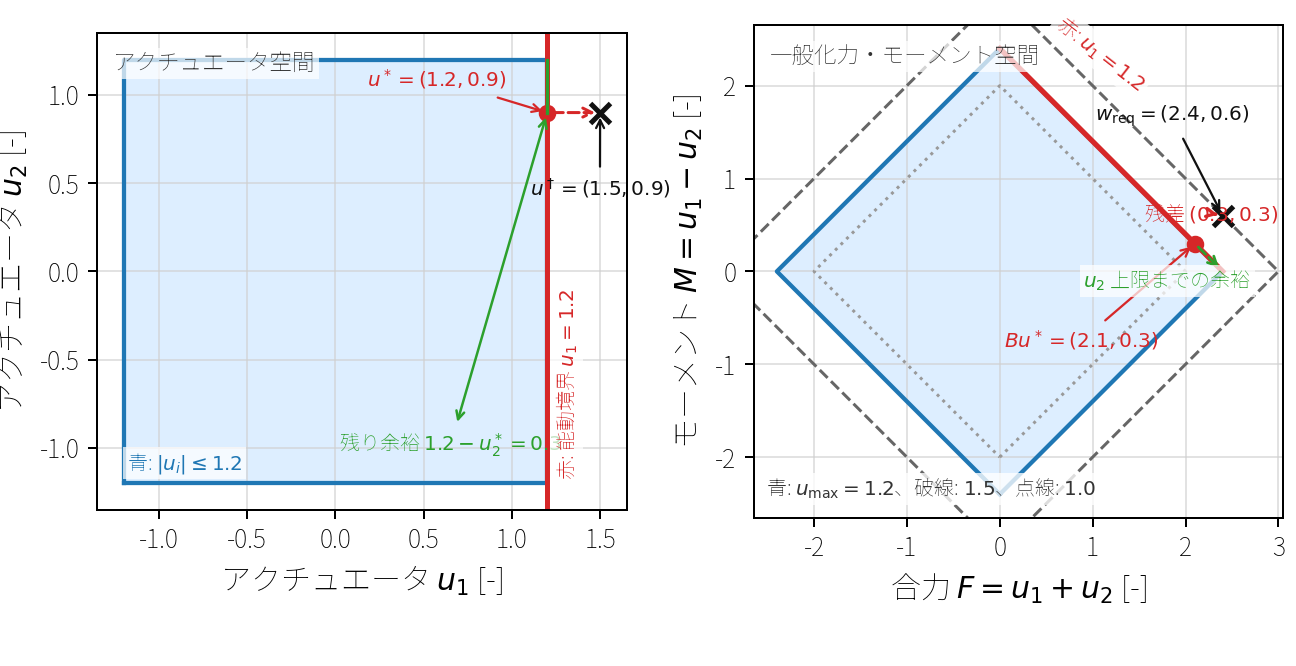
\includegraphics[width=0.96\linewidth,bb=0 0 1296 666]{figures/allocation_saturation_geometry.png}
  \caption{制御配分の飽和幾何。左はアクチュエータ空間で、制約なし配分 $u^\dagger=(1.5,0.9)^\T$ が上限 $u_1=1.2$ の外へ出ることを示す。右は同じ上限制約を合力 $F$ とモーメント $M$ の空間へ写した図であり、要求 $w_{\mathrm{req}}=(2.4,0.6)^\T$ は実現可能領域の外にある。飽和後の実現値は $Bu^*=(2.1,0.3)^\T$ で、赤い矢印が残差、緑の線分が第二入力側に残る余裕を表す。}
  \label{fig:allocation-saturation-geometry}
\end{figure}

能動集合を $u_1=u_{\max}=1.2$ と仮定すると、第二入力の停留条件は
\begin{align}
  \frac{\pp}{\pp u_2}
  \frac{1}{2}\norm{Bu-w_{\mathrm{req}}}^{2}
  &=
  \begin{bmatrix}1&-1\end{bmatrix}
  (Bu-w_{\mathrm{req}})=0,\\
  u_2^*&=\frac{F_{\mathrm{req}}-M_{\mathrm{req}}}{2}=0.9
\end{align}
である。したがって
\begin{equation}
  u^*=
  \begin{bmatrix}
    1.2\\0.9
  \end{bmatrix},
  \qquad
  Bu^*=
  \begin{bmatrix}
    2.1\\0.3
  \end{bmatrix},
  \qquad
  r_w=w_{\mathrm{req}}-Bu^*
  =
  \begin{bmatrix}
    0.3\\0.3
  \end{bmatrix}
\end{equation}
となる。第一入力の余裕は 0 で、第二入力には $u_{\max}-u_2^*=0.3$ の余裕が残る。合力もモーメントも要求値から $0.3$ ずつ不足しているので、この残差は「アクチュエータを丸めた」という実装上の注記ではなく、対象へ本当に届かなかった一般化指令である。

KKT 条件で見ると、この不足がどの境界に支えられているかが分かる。残差を
\begin{equation}
  e=Bu^*-w_{\mathrm{req}}
  =
  \begin{bmatrix}
    -0.3&-0.3
  \end{bmatrix}^\T
\end{equation}
とし、能動な上限制約だけを入れて
\begin{equation}
  \mathcal{L}(u,\mu_1)
  =
  \frac{1}{2}\norm{Bu-w_{\mathrm{req}}}^{2}
  +\mu_1(u_1-1.2)
\end{equation}
と置く。停留条件は
\begin{equation}
  B^\T e+
  \begin{bmatrix}
    \mu_1\\0
  \end{bmatrix}
  =
  \begin{bmatrix}
    -0.6\\0
  \end{bmatrix}
  +
  \begin{bmatrix}
    \mu_1\\0
  \end{bmatrix}
  =0
\end{equation}
であり、$\mu_1=0.6>0$、$\mu_1(u_1^*-1.2)=0$ となる。正の乗数は、要求点へ向かう残差をさらに減らす方向が、まさに $u_1$ 上限の外向き法線へ押し出されていることを示す。したがってログでは、$u^\dagger$ の上限超過量、実際に送った $u^*$、$Bu^*$、残差 $r_w$、能動境界、乗数、残り余裕を一組として残す必要がある。

上限を変えたときの変化も、同じ式で読める。
\begin{equation}
  \begin{array}{c|c|c|c|c}
    u_{\max}
    &u^*
    &Bu^*
    &w_{\mathrm{req}}-Bu^*
    &u_{\max}-u_2^*\\ \hline
    1.5
    &\begin{bmatrix}1.5\\0.9\end{bmatrix}
    &\begin{bmatrix}2.4\\0.6\end{bmatrix}
    &\begin{bmatrix}0\\0\end{bmatrix}
    &0.6\\
    1.2
    &\begin{bmatrix}1.2\\0.9\end{bmatrix}
    &\begin{bmatrix}2.1\\0.3\end{bmatrix}
    &\begin{bmatrix}0.3\\0.3\end{bmatrix}
    &0.3\\
    1.0
    &\begin{bmatrix}1.0\\0.9\end{bmatrix}
    &\begin{bmatrix}1.9\\0.1\end{bmatrix}
    &\begin{bmatrix}0.5\\0.5\end{bmatrix}
    &0.1
  \end{array}
\end{equation}
$u_{\max}=1.5$ では要求点は境界上にあり、第一入力の余裕はないが残差は 0 である。$u_{\max}=1.2$、$1.0$ と狭めると、図の実現可能な菱形領域が内側へ縮み、同じ要求点に対する残差が大きくなる。さらに $u_{\max}<0.9$ まで狭めると第二入力も能動になり、残差の向きは第一入力だけの法線では説明できなくなる。この変化を本文中の数値で追うことで、配分飽和は単なるクリップ処理ではなく、一般化力空間の可行領域、能動境界、残差、余裕を同時に変える制約付き最適化問題であることが確認できる。

\subsection{実装条件をモデルへ入れる}

\wfig{implementation-effects-examples} で確認した実装差は、最後に付ける補正ではなく、\wfig{mpc-architecture} の対象へ入る入力信号を定義し直す条件である。入力飽和を単なる注意として扱うと、理論と実機が離れる。計算入力を $u_{c,k}$、対象へ実際に入った入力を $u_k^{act}$ とおくと、飽和は
\begin{equation}
  u_k^{act}=\operatorname{sat}(u_{c,k}),\qquad
  x_{k+1}=A_dx_k+B_du_k^{act}
\end{equation}
と書ける。予測器が $u_{c,k}$ を使うと、同じ状態から出発しても一ステップ予測は
\begin{equation}
  \left(A_dx_k+B_du_{c,k}\right)
  -\left(A_dx_k+B_du_k^{act}\right)
  =B_d\left(u_{c,k}-u_k^{act}\right)
\end{equation}
だけずれる。飽和していない区間ではこの差は 0 だが、\wfig{implementation-effects-examples} の赤線のように上限または下限に当たる区間では、差分 $u_{c,k}-u_k^{act}$ がそのままモデル化された外乱のように予測へ入る。したがって、推定器の時間更新も
\begin{equation}
  \hat{x}_{k+1|k}=A_d\hat{x}_{k|k}+B_du_k^{act}
\end{equation}
で行い、$u_{c,k}$ ではなくログに残した実入力を用いる。そうすれば、観測残差はセンサ雑音やモデル誤差を表し、既知の飽和差を推定誤差へ混ぜない。

レート制限も同じ構造である。サンプル間で動かせる入力変化を $\Delta u_{\max}$ とすると、実入力は
\begin{equation}
  u_k^{act}
  =u_{k-1}^{act}
  +\operatorname{clip}
  \left(u_{c,k}-u_{k-1}^{act},-\Delta u_{\max},\Delta u_{\max}\right)
\end{equation}
であり、対象の更新式はやはり $x_{k+1}=A_dx_k+B_du_k^{act}$ になる。ここでも $u_{c,k}$ をそのまま予測へ入れた場合のずれは $B_d(u_{c,k}-u_k^{act})$ であり、制限が能動になった瞬間だけ、予測と観測の差が実装条件によって生じる。

一サンプル遅れでは、サンプル $k$ で計算または制限された入力は次の区間まで対象へ届かない。したがって対象が区間 $[k,k+1)$ で見る入力は現在の $u_{c,k}$ ではなく直前に適用済みの $u_{k-1}^{act}$ であり、
\begin{equation}
  x_{k+1}=A_dx_k+B_du_{k-1}^{act}
\end{equation}
となる。過去入力を状態へ含めると
\begin{equation}
  \xi_k=\begin{bmatrix}x_k\\u_{k-1}^{act}\end{bmatrix}
\end{equation}
として
\begin{equation}
 \xi_{k+1}=\begin{bmatrix}A_d&B_d\\0&0\end{bmatrix}\xi_k+
  \begin{bmatrix}0\\I\end{bmatrix}u_k^{act}
\end{equation}
を得る。これは経験的な補正ではなく、遅れを含む対象を別の状態空間モデルへ書き直した結果である。MPC がこの拡大モデルで予測を始める初期条件は、推定した対象状態だけでは足りない。各サンプルの初期条件は
\begin{equation}
  \xi_{k|k}=
  \begin{bmatrix}
    \hat{x}_{k|k}\\
    u_{k-1}^{act}
  \end{bmatrix}
\end{equation}
であり、最後に対象へ適用された入力を状態と同じ時刻情報として保存しておく必要がある。遅れが複数サンプルにまたがる場合や入力キューを持つ実装では、初期条件に含める対象はさらに増え、キューに保持されている適用済みまたは適用予定の実入力列と、サンプル時刻やキューの進み具合を表すタイミング状態を、予測モデルと観測器の両方へ同じ順序で渡す。こうして \wfig{implementation-effects-examples} の計算入力と実入力のずれは、後処理の注釈ではなく、MPC の状態、入力、制約余裕を決めるモデルの一部になる。
